%% Plato FSM Translation Tech Memo
%% FSM background
\newpage
\section {Finite State Machines \label {sec:fsms}}

Finite State Machines can be used to model behaviour of all levels of system~\cite{Taraate2016}. 
The formalism contains states, which are the vertices, and transitions between these states, which 
are the arcs. Applied to each transition is the event for that transition to occur, causing a change 
of state. Depending on the level of system that is being modelled, this event can be a condition being met,
such as the temperature being over a certain value, or it could be a signal transition. 

Regardless of system level, an FSM model always shows some key parts of the system. Each state a system is 
in usually has an associated output or action, which occurs upon entry to this state and continues while the system remains
in this state, and when an event occurs, the state will change depending on what state the system is in, and which event occured. 

For example, Figure~\ref{fig:stopwatch} contains the example FSM which models the 
high-level behaviour of a stopwatch.

\begin{figure}[h]
\begin{centering}
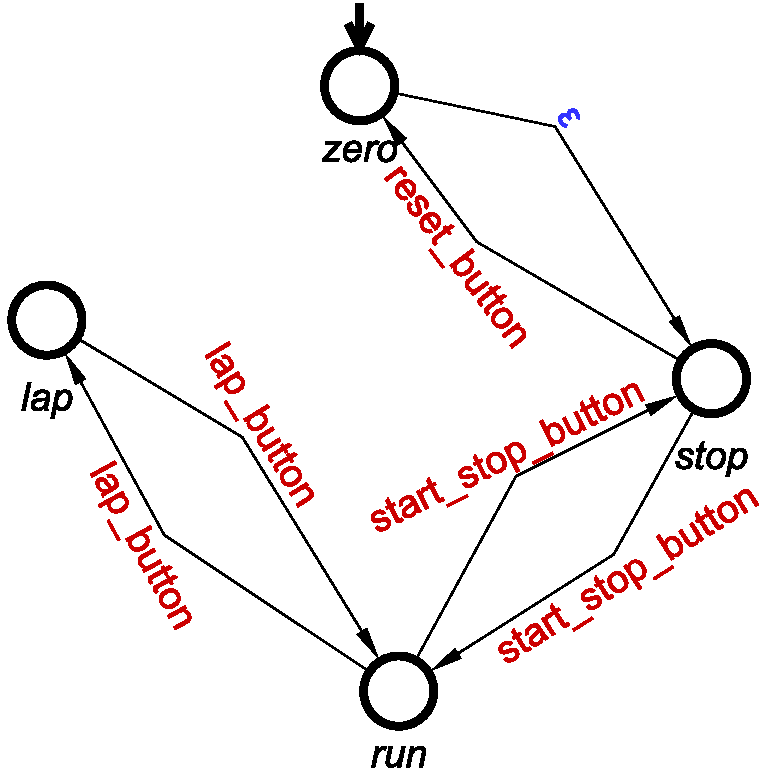
\includegraphics[scale=0.5]{images/stopwatch-fsm}
\par\end{centering}
\protect\caption{\label{fig:stopwatch} Stopwatch FSM}
\end{figure}

\noindent There are four states, which are:

\begin{itemize}

\item Zero - The initial state, where the timer and display are reset to 0. 

\item Stop - In this state, the timer and display are paused.

\item Run - While in this state, the timer is counting, and the display shows this.

\item Lap - In this state, the timer continues counting but the display shows the time when lap was entered.

\end{itemize}

\noindent The transitions between these are based on three buttons:

\begin{itemize} 

\item Reset button - When it has been stopped (in the stop state), moves the system to the zero state to reset everything to 0.

\item Start/Stop button - Used to move the stopwatch from the stop state to the run state, and back. This starts and pauses the timer. 

\item Lap button - This moves the system from the run state, to the lap state, to hold a time on the display for recording. 
                              Also moves it back to the run state, updating the display to the actual time
                              
\end{itemize}

\noindent Also, not that when the zero state is reached, there is an $\varepsilon$ symbol. This symbol represents that
a transition occurs without any requirements. For this example, it is important, as when the system initialises or is reset, we 
want the display and counter to be set to 0, and following this, be ready to start counting. This therefore resets the system, and
moves into the stop state, ready for the timer to being counting from a start/stop button press. 

This is a high-level model as it describes the possible states of the system, but not the low-level implementation details. 
For example, we know what buttons to press to move between states, but there is nothing to say what constitues a button ``press'', 
and, while we know how the display should react depending on the state, we have not provided any details on how we control the display. 

The stopwatch behaviour however does identify the key parts. Each state has an associated action, which we have described. Each transition
has an associated event, these being either button presses, or nothing. We also know that for each state, we can transition to a new state if a
specific button is pressed, but if that button is not associated with a transition from the current state, the state will remain the same, for example, 
if we press the reset button while in the run state, we cannot changes state. 

This example can be used further by adding some implementation details, based on how the components, the buttons and display, work, yet 
the behaviour of the stop-watch will remain the same. 

FSMs can be used to model circuits at the signal-level, as with STGs. In this case, the actions associated with the states can be simply the
arrangement of the signals in the system, the effect of this arrangment causing changes in the environment of the circuit itself. The events 
associated with the transitions between states can be signal transitions. For example, Figure~\ref{fig:handshake-fsm} contains a handshake FSM.

\begin{figure}[h]
\begin{centering}
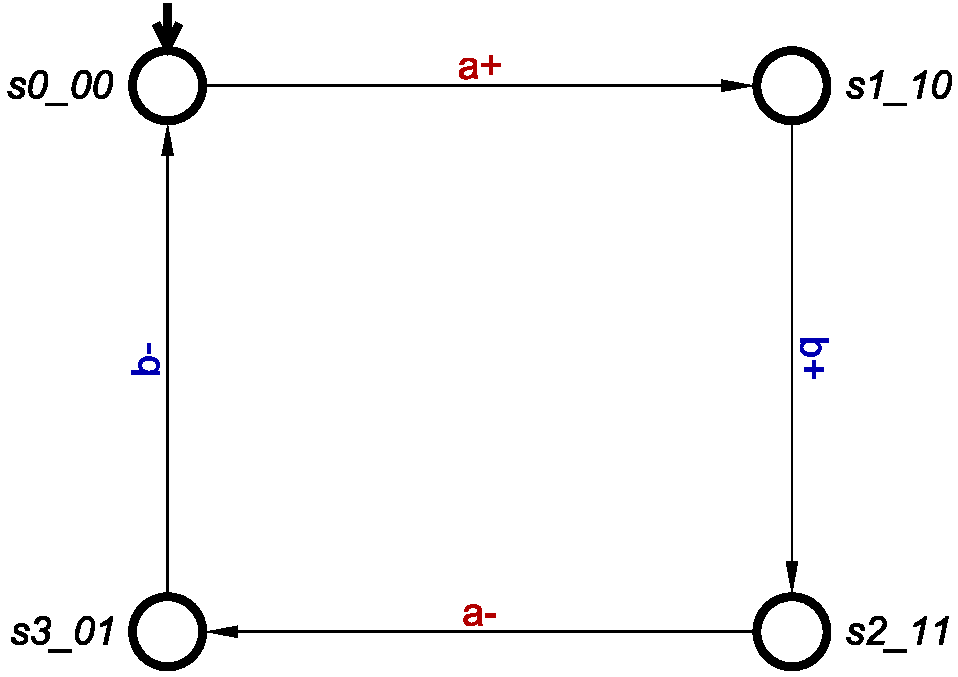
\includegraphics[scale=0.5]{images/handshake-fsm}
\par\end{centering}
\protect\caption{\label{fig:handshake-fsm} Handshake FSM}
\end{figure}

In this example there is one input signal, $a$, one output signal, $b$, and four states: 

\begin{itemize}

\item 00 - The initial state, where both input and output have transitioned low.

\item 10 - The input has gone from 0 to 1.

\item 11 - The output transitions from 0 to 1.

\item 01 - The input transitions low, from 1 to 0.

\end{itemize}

\noindent The transitions between feature the events of these signals transitioning high and low. 

In this case, we have included the implementation details, specifically in what signal transitions cause a changes of state, 
therefore this can be considered a low-level FSM model. However, this doesn't change the fact that the key behaviours are identified. 

Since FSMs can be used generally at all different levels of behavioural modelling, the requirements for what constitutes and event for
a state transition, are not stated, therefore, as with these examples they can be a button press or a signal transition. There exists 
a form of FSM specifically designed for modelling circuit behaviour at signa-level, such as in Figure~\ref{fig:handshake-fsm} named 
\emph{Finite State Transducers} (FSTs). 

FSTs aim to be used for specifications of circuits, and can be used for specifying asynchronous circuits. They allow signals
to be set as specific types, inputs, outputs and internals for example, but do not differ in how they show behaviours. For this reason, 
they can be converted to and from other modelling methods aimed at showing signal-level behaviours such as STGs, and this applies
to \noun{Plato}, where a concept specification must be able to produce either an FSM or an STG without any changes to the specification. 

When using \noun{Workcraft}, an STG can be translated from a concept specification using \noun{Plato} from the STG plugin, and while \noun{Workcraft} does
feature both an FSM and FST plugin, for the interoperability of STGs and FSTs, a concept specification can be translated only to an FST. For this paper however, 
we will continue to FSTs translated from concepts as FSMs. 

\subsection{FSMs and STGs \label{sub:FSMs-STGs}}

As with Signal Transition Graphs, Finite State Machines can be used to model the behaviour of asynchronous circuits at the signal level. However,
the methods that they use to show the interactions between signals are quite varied. There are similarities, for example, Figure~\ref{fig:handshakes-all}
shows a handshake in both STG and FSM form.

\begin{figure}[H]
\subfigure[Handshake in FSM form] {
  \centering
  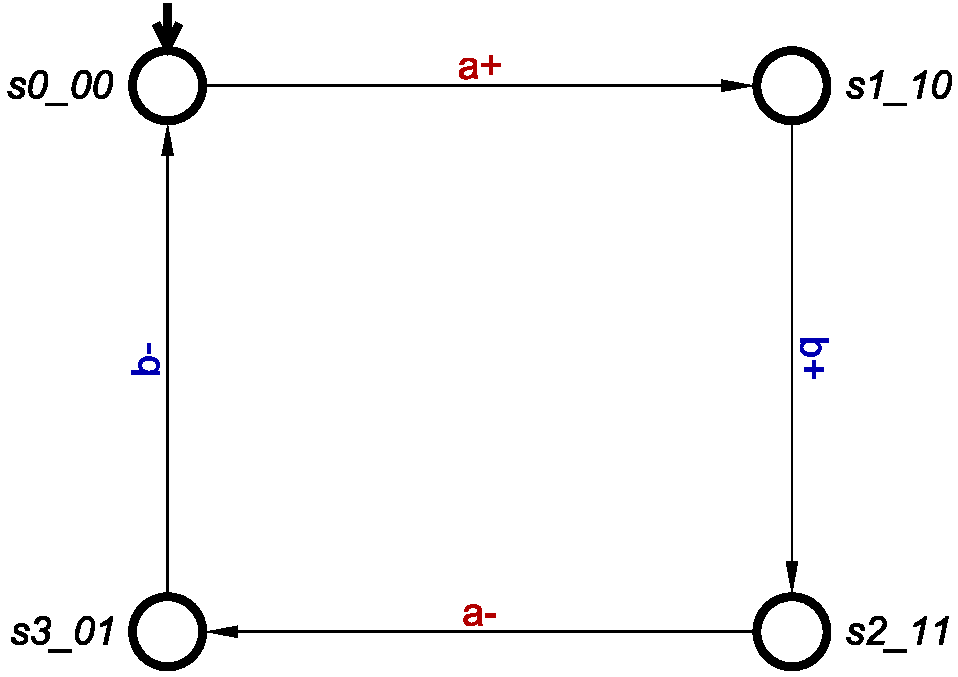
\includegraphics[scale=0.5]{images/handshake-fsm}
  \label{fig:handshakes-all-fsm}
  }
\subfigure[Handshake in STG form] {
  \centering
  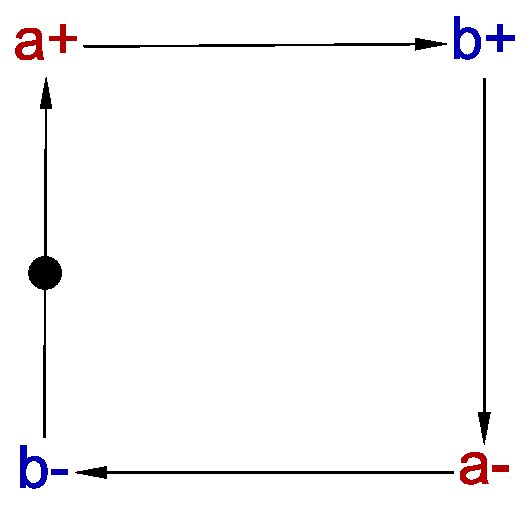
\includegraphics[scale=0.64]{images/handshake-stg}
  \label{fig:handshakes-all-stg}
  }
  \caption{\label{fig:handshakes-all} Handshakes in both FSM and STG format}
\end{figure}

The FSM handshake~(Figure~\ref{fig:handshakes-all-fsm}) and the STG handshake~(Figure~\ref{fig:handshakes-all-stg}) are both in a 
square shape, indicating that there are two signals involved, horizontal transitions indicate one signal's transitions, and vertical transitions 
indicating the other. These are fairly simple structures in both modelling formalism however. 

The major differences between these modelling methods are shown when concurrency comes into play. When two or more signals are
set to transition in the same period, i.e. one signal transition causes two other signal transitions, the latter two not having any
strict requirements on the orders they transition. 

To demonstrate the differences, let's use the example of a C-element with environment. In this example, there are three signals, 
$a$ and $b$ are inputs signals, and $c$ is an output signal. $a$ and $b$ are the input signals to a C-element, the output of which is $c$. 
The environment is composed of two inverters, both inputs of which are signal $c$, and the output of one is signal $a$, the other is signal $b$. 
If we model these as both an FSM and an STG, we are provided with the models as seen in Figure~\ref{fig:c-element-env}.

\begin{figure}[H]
\subfigure[A C-Element with environment in FSM form] {
  \centering
  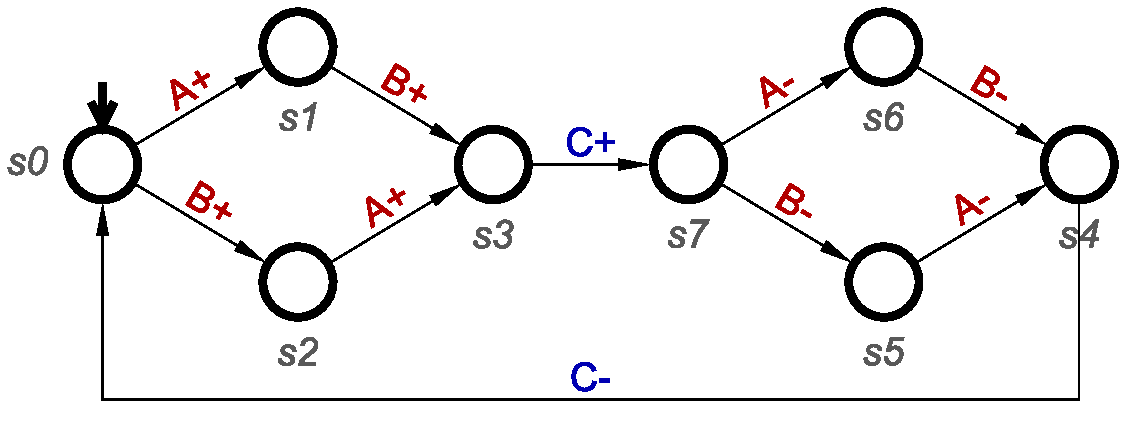
\includegraphics[scale=0.45]{images/c-element-env-fsm}
  \label{fig:c-element-env-fsm}
  }
\subfigure[A C-element with environment in STG form] {
  \centering
  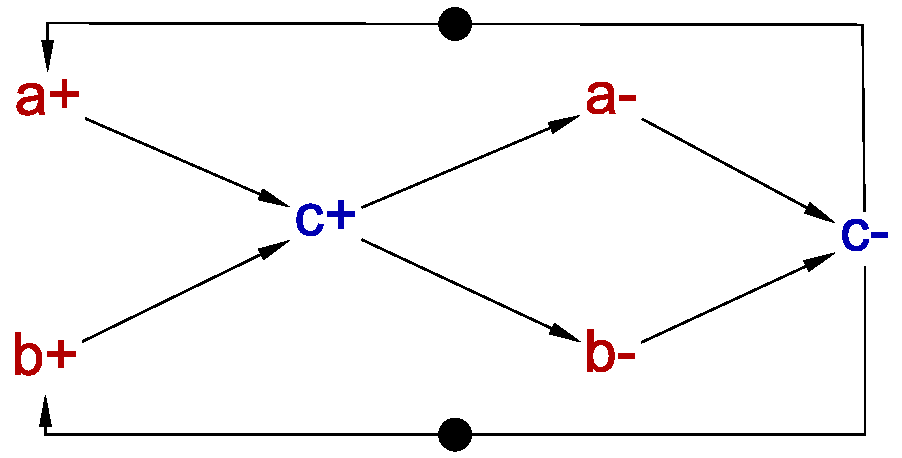
\includegraphics[scale=0.4]{images/c-element-env-stg}
  \label{fig:c-element-env-stg}
  }
  \caption{\label{fig:c-element-env} C-Element with environment example in both FSM and STG format}
\end{figure}

Both of these models, FSM in Figure~\ref{fig:c-element-env-fsm}, STG in Figure~\ref{fig:c-element-env-stg}, feature structures 
where the transitions ``expand''. For example, in both models after the $c^{+}$ transition, the following transitions are ``expanded''. 
This structure indicates concurrency in both models. However, what these expansions show is different in either model. 

In the STG, there are two transitions in the expansion, $a^{-}$ and $b^{-}$, one on each branch and this shows that the transitions
 occur concurrently, and either can occur before the other. However, for the transition following these, $c^{-}$, both must occur.
In the FSM, each branch features both possible orders of both signals, $a^{-}$ then $b^{-}$, or $b^{-}$ then $a^{-}$, which must occur
for $c^{-}$ to occur. It could be argued that in the FSM of this example, the concurrency it shows indiciates more explicitly that either order of the
signal transitions can occur, which may be preferable in some cases. However, the STG model does not contain the states and thus looks
cleaner and simpler.

The concurrency in this example is fairly minimal, and the resulting expansions in both models are
similar. The differences become more apparent when the number of concurrent signal transitions increases. 
 
\begin{figure}[H]
	\centering
	\subfigure[An example with 3 concurrent signals in FSM form] {
		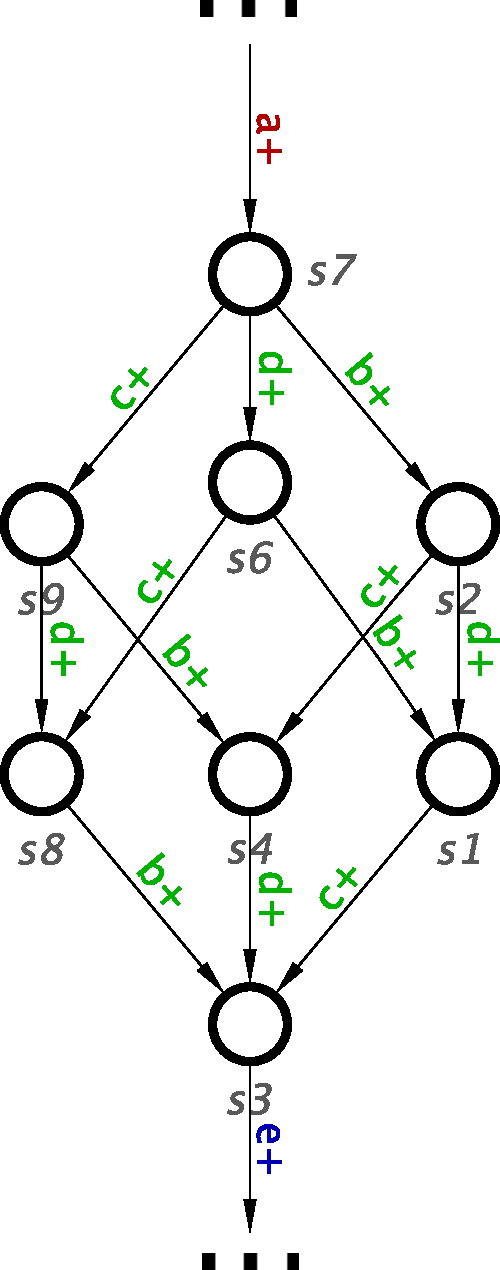
\includegraphics[scale=0.4]{images/concurrency-fsm}
		\label{fig:concurrency-fsm}
	}
\hspace{10mm}
	\subfigure[An example with 3 concurrent signals in STG form] {
		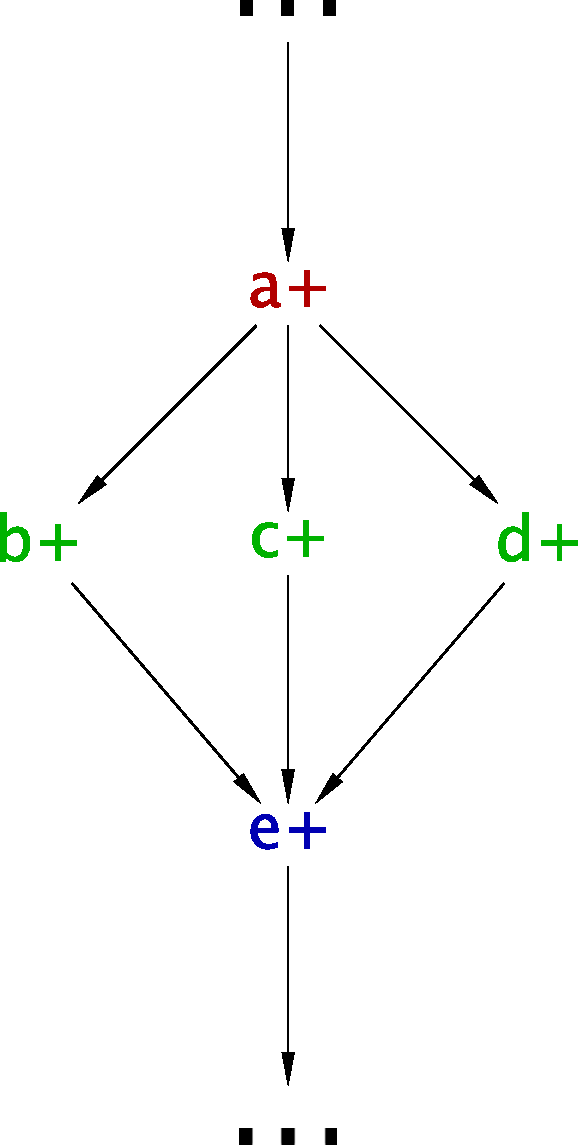
\includegraphics[scale=0.4]{images/concurrency-stg}
		\label{fig:concurrency-stg}
	}
	\caption{\label{fig:concurrency-example} An example with 3 concurrent signal transitions}
\end{figure} 

Figure~\ref{fig:concurrency-example} is an example of both model formalisms containing three 
concurrent signal transitions. Each one is a snippet, and does not feature the whole model. 
Figure~\ref{fig:concurrency-fsm} is the FSM form of this example, and as with the previous example, 
this contains every possible order that these three signals can transition in, and this has lead to a wide 
expansion, with arcs crossing over each other. In comparison, the expansion of the STG form, shown in 
Figure~\ref{fig:concurrency-stg}, has much less expansion, with the three transitions all requiring to 
have occurred, for a "join" where $e^{+}$ can occur. 

In an example of this size, it is still relatively clear in both the FSM and STG how these signals can 
transition concurrently, however, as the number of concurrent signals increase, the size of the 
expansion in the FSM will also increase, leading to further arcs which will cross over, and make 
comprehension of such a model more difficult. 

The size of an FSM in comparison to an STG is not simply dictated by the number of concurrent signals 
in a snippet, however. Due to the encoding of the states, which is based on the states of the signals, 
meaning that an FSM can have $2^{n}$ possible states, where $n$ is the number of signals. It may be
that not every possible state is reachable, but this can still mean that there are many states. 

This phenomenon is known as \emph{state explosion}, meaning that where an STG may be able to 
model behaviours, the FSM equivalent can have so many possible states that traversing it can be 
computationally difficult. This is why STGs are preferred when modelling asynchronous systems, which 
contain a lot of concurrency, and may have many signals. 

As such, if a user chooses to translate a concept specification to an FSM to view it's intricacies and 
possible ordering of signals, it is recommended that this is performed on smaller specifications, or on 
smaller scenarios of a concept specification, which can be composed with other scenarios for a full 
concept specification.
 